\documentclass{beamer}

\author{作者姓名}
\title{主标题}
\subtitle{副标题}
\institute{华南理工大学}
\date{\today}

\usepackage{ctex, hyperref}
\usepackage[T1]{fontenc}
\usepackage{latexsym,amsmath,xcolor,multicol,booktabs,calligra}
\usepackage{graphicx,pstricks,listings,stackengine}
\usepackage{scutstyle}
\usepackage{cite}

\usefonttheme[onlymath]{serif}

\def\cmd#1{\texttt{\color{red}\footnotesize $\backslash$#1}}
\def\env#1{\texttt{\color{blue}\footnotesize #1}}
\definecolor{deepblue}{rgb}{0,0,0.5}
\definecolor{deepred}{rgb}{0.6,0,0}
\definecolor{deepgreen}{rgb}{0,0.5,0}
\definecolor{halfgray}{gray}{0.55}

\lstset{
    basicstyle=\ttfamily\small,
    keywordstyle=\bfseries\color{deepblue},
    emphstyle=\ttfamily\color{deepred},
    stringstyle=\color{deepgreen},
    numbers=left,
    numberstyle=\small\color{halfgray},
    rulesepcolor=\color{red!20!green!20!blue!20},
    frame=shadowbox,
}



\begin{document}

\kaishu
\begin{frame}
    \begin{figure}[htpb]
        \begin{center}
            
\includegraphics[width=0.5\linewidth]{img/scut-logo-2.png}
        \end{center}
    \end{figure}
    \titlepage
\end{frame}

\begin{frame}
    \tableofcontents[sectionstyle=show,subsectionstyle=show/shaded/hide,subsubsectionstyle=show/shaded/hide]
\end{frame}



\section{样式示例}

\begin{frame}{自定义标题}
    \begin{enumerate}
        \item 这是一句
        \item 分开的 \newline 话。
    \end{enumerate}
\end{frame}

\subsection{样式示例}

\begin{frame}{再来一次}
    \begin{itemize}[<+-| alert@+>]
        \item 这又是
        \item 一句话 \cite{Doe2022}
    \end{itemize}
\end{frame}

\section{关于Beamer}

\begin{frame}{表格示例}
    \begin{itemize}
        \item \LaTeX 广泛用于学术界,期刊会议论文模板
    \end{itemize}
    \begin{table}[h]
        \centering
        \caption{二者比较}
        \label{tab:camparison}
        \begin{tabular}{c|c}
            Microsoft\textsuperscript{\textregistered}  Word & \LaTeX \\
            \hline
            文字处理工具 & 专业排版软件 \\
            所见即所得 & 一门“编程语言” \\
        \end{tabular}
    \end{table}
\end{frame}

\begin{frame}{排版示例}
    \begin{exampleblock}{无编号公式}
        \begin{equation*}
            F=ma
        \end{equation*}
    \end{exampleblock}
    \begin{block}{和差化积公式,多行}
        \begin{equation}
            \label{hecha1}
            \sin x + \sin y = 2\sin \frac{x+y}{2} \cos \frac{x-y}{2} \nonumber
        \end{equation}
        \begin{equation}
            \label{hecha2}
            \sin x - \sin y = 2\cos \frac{x+y}{2} \sin \frac{x-y}{2}
        \end{equation}
        \begin{equation}
            \label{hecha3}
            \cos x + \cos y = 2\cos \frac{x+y}{2} \cos \frac{x-y}{2}
        \end{equation}
        \begin{equation}
            \label{hecha4}
            \cos x - \cos y = -2\sin \frac{x+y}{2} \sin \frac{x-y}{2}
        \end{equation}
    \end{block}
\end{frame}

\begin{frame}
    \begin{exampleblock}{编号多行公式}
        \begin{multline}
            A=\lim_{n\rightarrow\infty}\Delta x\left(a^{2}+\left(a^{2}+2a\Delta x+\left(\Delta x\right)^{2}\right)\right.\label{eq:reset} \\
            +\left(a^{2}+2\cdot2a\Delta x+2^{2}\left(\Delta x\right)^{2}\right) \\
            +\left(a^{2}+2\cdot3a\Delta x+3^{2}\left(\Delta x\right)^{2}\right) \\
            +\ldots\\
            \left.+\left(a^{2}+2\cdot(n-1)a\Delta x+(n-1)^{2}\left(\Delta x\right)^{2}\right)\right) \\
            =\frac{1}{3}\left(b^{3}-a^{3}\right)
        \end{multline}
    \end{exampleblock}
\end{frame}

\begin{frame}{图形与分栏}
    \begin{minipage}[c]{0.3\linewidth}
        \psset{unit=0.8cm}
        \begin{pspicture}(-1.75,-3)(3.25,4)
            \psline[linewidth=0.25pt](0,0)(0,4)
            \rput[tl]{0}(0.2,2){$\vec e_z$}
            \rput[tr]{0}(-0.9,1.4){$\vec e$}
            \rput[tl]{0}(2.8,-1.1){$\vec C_{ptm{ext}}$}
            \rput[br]{0}(-0.3,2.1){$\theta$}
            \rput{25}(0,0){%
            \psframe[fillstyle=solid,fillcolor=lightgray,linewidth=.8pt](-0.1,-3.2)(0.1,0)}
            \rput{25}(0,0){%
            \psellipse[fillstyle=solid,fillcolor=yellow,linewidth=3pt](0,0)(1.5,0.5)}
            \rput{25}(0,0){%
            \psframe[fillstyle=solid,fillcolor=lightgray,linewidth=.8pt](-0.1,0)(0.1,3.2)}
            \rput{25}(0,0){\psline[linecolor=red,linewidth=1.5pt]{->}(0,0)(0.,2)}
%           \psRotation{0}(0,3.5){$\dot\phi$}
%           \psRotation{25}(-1.2,2.6){$\dot\psi$}
            \psline[linecolor=red,linewidth=1.25pt]{->}(0,0)(0,2)
            \psline[linecolor=red,linewidth=1.25pt]{->}(0,0)(3,-1)
            \psline[linecolor=red,linewidth=1.25pt]{->}(0,0)(2.85,-0.95)
            \psarc{->}{2.1}{90}{112.5}
            \rput[bl](.1,.01){C}
        \end{pspicture}
    \end{minipage}\hspace{1cm}
    \begin{minipage}{0.5\linewidth}
        \medskip
        %\hspace{2cm}
        \begin{figure}[h]
            \centering
            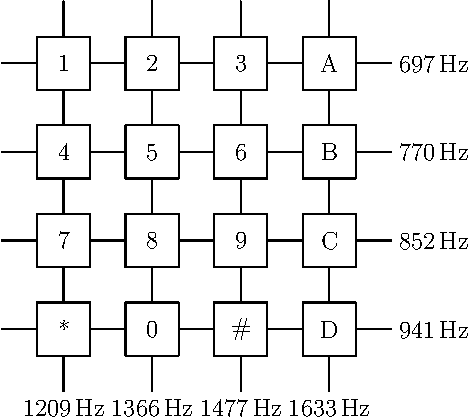
\includegraphics[height=.4\textheight]{img/dtmf.pdf}
        \end{figure}
    \end{minipage}
\end{frame}

\begin{frame}[fragile]{\LaTeX{} 常用命令}
    \begin{exampleblock}{命令}
        \centering
        \footnotesize
        \begin{tabular}{llll}
            \cmd{chapter} & \cmd{section} & \cmd{subsection} & \cmd{paragraph} \\
            章 & 节 & 小节 & 带题头段落 \\\hline
            \cmd{centering} & \cmd{emph} & \cmd{verb} & \cmd{url} \\
            居中对齐 & 强调 & 原样输出 & 超链接 \\\hline
            \cmd{footnote} & \cmd{item} & \cmd{caption} & \cmd{includegraphics} \\
            脚注 & 列表条目 & 标题 & 插入图片 \\\hline
            \cmd{label} & \cmd{cite} & \cmd{ref} \\
            标号 & 引用参考文献 & 引用图表公式等\\\hline
        \end{tabular}
    \end{exampleblock}
    \begin{exampleblock}{环境}
        \centering
        \footnotesize
        \begin{tabular}{lll}
            \env{table} & \env{figure} & \env{equation}\\
            表格 & 图片 & 公式 \\\hline
            \env{itemize} & \env{enumerate} & \env{description}\\
            无编号列表 & 编号列表 & 描述 \\\hline
        \end{tabular}
    \end{exampleblock}
\end{frame}

\begin{frame}[fragile]{\LaTeX{} 环境命令举例}
    \begin{minipage}{0.5\linewidth} % 下面注意缩进!
        \begin{lstlisting}[language=TeX]
\begin{itemize}
    \item A \item B
    \item C
    \begin{itemize}
        \item $C-1$
    \end{itemize}
\end{itemize}
        \end{lstlisting}
    \end{minipage}\hspace{1cm}
    \begin{minipage}{0.3\linewidth}
        \begin{itemize}
            \item A
            \item B
            \item C
            \begin{itemize}
                \item $C-1$
            \end{itemize}
        \end{itemize}
    \end{minipage}
    \medskip
    \pause
    \begin{minipage}{0.5\linewidth}
        \begin{lstlisting}[language=TeX]
\begin{enumerate}
    \item 巨佬
    \item 蒟蒻
    \begin{itemize}
      \item[n+e] 瑟瑟发抖
    \end{itemize}
\end{enumerate}
        \end{lstlisting}
    \end{minipage}\hspace{1cm}
    \begin{minipage}{0.3\linewidth}
        \begin{enumerate}
            \item 巨佬
            \item 蒟蒻
            \begin{itemize}
                \item[n+e] 瑟瑟发抖
            \end{itemize}
        \end{enumerate}
    \end{minipage}
\end{frame}

\begin{frame}[fragile]{\LaTeX{} 数学公式}
    \begin{columns}
        \begin{column}{.55\textwidth}
            \begin{lstlisting}[language=TeX]
$V = \frac{4}{3}\pi r^3$
\[
    V = \frac{4}{3}\pi r^3
\]
\begin{equation}
    \label{eq:vsphere}
    V = \frac{4}{3}\pi r^3
\end{equation}
            \end{lstlisting}
        \end{column}
        \begin{column}{.4\textwidth}
            $V = \frac{4}{3}\pi r^3$
            \[
                V = \frac{4}{3}\pi r^3
            \]
            \begin{equation}
                \label{eq:vsphere}
                V = \frac{4}{3}\pi r^3
            \end{equation}
        \end{column}
    \end{columns}
\end{frame}

\begin{frame}{作图}
    \begin{itemize}
        \item 矢量图 eps, ps, pdf
        \begin{itemize}
            \item METAPOST, pstricks, pgf $\ldots$
            \item Xfig, Dia, Visio, Inkscape $\ldots$
            \item Matlab / Excel 等保存为 pdf
        \end{itemize}
        \item 标量图 png, jpg, tiff $\ldots$
        \begin{itemize}
            \item 提高清晰度,避免发虚
            \item 应尽量避免使用
        \end{itemize}
    \end{itemize}
    \begin{figure}[htpb]
        \centering
        
\includegraphics[width=0.2\linewidth]{img/scut-logo.jpg}
        \caption{校徽}
    \end{figure}
\end{frame}

\section{参考文献}

\begin{frame}[allowframebreaks]
    \bibliographystyle{alpha}
    \bibliography{ref}
    % 参考文献太多,可以这样调整字体:\tiny\bibliographystyle{alpha}
\end{frame}

\begin{frame}
    \begin{center}
        {\Huge\calligra Thanks!}
    \end{center}
\end{frame}

\end{document}
